\section{Meilenstein 4: Spawning, Kollisionen und $N+1$}\label{sec:meilenstein_4}

Meilenstein 4 sah die Fertigstellung eines \textit{Vertical Slice} vor, in dem die wichtigsten Regeln und Mechaniken des Spiels implementiert werden sollten.\\

Da sich die vorherigen Meilensteine vor allem auf die technische Umsetzung des Framework-Grundgerüsts konzentriert hatten, sah sich die Entwicklung zu diesem Zeitpunkt mit der Herausforderung konfrontiert, die mit Meilenstein 3 begonnenen und zunehmend komplexer werdenden Spielmechaniken zu integrieren.
Dies machte eine umfassende Umstrukturierung der Codebasis erforderlich.
Abgeschlossen werden konnte der Meilenstein schließlich mit einer API für die \textit{GameLoop}, die eine klarere Strukturierung der verschiedenen Systeme innerhalb einer Frame-Iteration erlaubte (siehe Abschnitt~\ref{sec:runtime_gameloop}).
Insgesamt wurden in diesem Meilenstein folgende Konzepte umgesetzt:

\begin{itemize}
    \itemsep0.5em
    \item Einführung des \texttt{Manager}-Konzepts als Orchestrator spezifischer Subsysteme (siehe Abschnitt~\ref{sec:runtime_manager}).
    \item Entwurf einer \textit{phasenbasierten} \textit{GameLoop}, die mit verschiedenen \textit{Passes} und \textit{Commit Points} klare Schnittstellen für Systemübergänge definiert.
    \item Implementierung von \texttt{CommandHandler} und \texttt{CommandBuffer}, die nach dem \textit{Push-Pull}-Prinzip verschiedene Phasen der \textit{GameLoop} zum Nachrichtenaustausch nutzen können.
\end{itemize}

Die bereits erwähnte Umstrukturierung der Codebasis hatte indes auch Auswirkungen auf den Entwicklungsprozess:
Die im Prototyp-Dokument erwähnte strikte Trennung in \textit{Module Interface Units} und \textit{Implementation Units}~\cite[S. 211-213]{Str24} wurde zugunsten eines verbesserten Refactoring-Workflows aufgegeben.
Die Implementierungen wurden in die eigentlichen \textit{Interface Units} zurückgeführt (\textit{Header-only}-Ansatz~\cite[S. 279]{Wil05}).
Ein wesentlicher Grund hierfür war das im Rahmen der iterativen Entwicklung typische Refactoring.
Die Aufteilung führte trotz ausreichender IDE-Unterstützung\footnote{
    CLion, \url{https://www.jetbrains.com/clion}, Abrufdatum 13.03.2026
} zu einer spürbaren kognitiven Last:
Häufige Kontextwechsel bei der Navigation durch die Quelldateien verzögerten die Anpassung von Schnittstellendefinition und zugehöriger Implementierung.\footnote{
    Studien zu kognitiver Last in der Softwareentwicklung finden sich unter anderem bei Helgesson et al.~\cite{HERB19}, die Entwicklerwerkzeuge als Belastungsfaktor identifizieren, sowie bei Gonçalves et al.~\cite{GSFF19}, die Auswirkungen kognitiver Belastung auf die Arbeitsqualität untersuchen.
}
Die Auswirkungen auf die Kompilierzeit wurden im Projektkontext als vernachlässigbar eingestuft, wobei eine belastbare Messung an dieser Stelle aussteht.


\subsubsection{Expression Builder für das Spawn-System}
Außerdem erfolgte eine logische Trennung zwischen engine-intrinsischen Funktionen - der bereits zitierten \textit{Runtime} - und Modulen, die für Spielmechaniken verantwortlich sind.
Zwischen diesen (\texttt{mechanics}) besteht ein äußerst geringer Grad an Kopplung; sie stellen unter anderem Implementierungen für Kampf- und Punktesysteme bereit.
Zudem wurde ein \textit{policy-basiertes} System für Spawning und Despawning eingeführt, das auf dem im \texttt{runtime}-Modul platzierten Spawn-System von \textit{helios} aufsetzt.
Dieses wurde im weiteren Verlauf ausgebaut und kann mithilfe einer \textit{Domain Specific Language} (DSL) konfiguriert werden, um eine semantische Konfiguration von Spawn-Logiken in Verbindung mit \textit{Prefab}-Pools vorzunehmen.\\

Der in diesem Zusammenhang implementierte \textit{Expression Builder}~\cite[S. 343-350]{FP11} erlaubt die Konfiguration von \texttt{GameObject}s wie Spielern, Gegnern, Projektilen und Spielfiguren.
Mit dieser Factory lässt sich der Code zur Spielweltkonfiguration einfacher und lesbarer halten.
Außerdem müssen semantische Details nicht in der abstrakteren Implementierung aufgenommen werden (siehe Listing~\ref{lst:gameobjectdsl}).\\

\begin{lstlisting}[style=c++style,
    caption={Auszug aus dem Code zur Konfiguration des \textit{BlueEnemy}, einem Gegnertyp, der 30 Sekunden nach Spielbeginn in der \textit{Collision Detection Demo} spawnt und aus einer Chase-Komponente zum Verfolgen des Spielers besteht.},
    label=lst:gameobjectdsl]
    auto blueEnemyPrefab = GameObjectFactory::instance()
        .gameObject()
        .withCollision([](auto& cb) {
            cb.collision()
              .layerId(CollisionId::Enemy)
              .useBoundingBox()
              .onSolidCollision(CollisionId::Player, CollisionBehavior::Despawn)
              .onSolidCollision(CollisionId::Projectile, CollisionBehavior::Despawn);
        })
        .withAi([&](auto& aib) {
            aib.chasing()
               .target(shipGameObject->guid())
               .seekInterval(0.05f);
        })
       .make();
\end{lstlisting}

Dem Code in Listing~\ref{lst:gameobjectdsl} ist die \textit{vanilla} Konfiguration eines \texttt{GameObject} gegenübergestellt (siehe Listing~\ref{lst:gameobjectcmpbased}).
Im direkten Vergleich lässt sich erkennen, dass die Gruppierung von Komponenten hinter einfacher lesbaren Methoden, die über ein \textit{Fluent Interface}~\cite{FluentInterface} realisiert wurden, den Quellcode zwar nicht wesentlich reduziert, ihn aber intuitiv verständlicher macht.

\begin{lstlisting}[style=c++style,
    caption={Konfiguration eines Spieler-Objekts ohne DSL (Codebasis Meilenstein 4).},
    label=lst:gameobjectcmpbased]
auto shipGameObject = std::make_unique<GameObject>();
shipGameObject->add<SceneNodeComponent>(spaceshipSceneNode);
shipGameObject->add<TwinStickInputComponent>();
// ... weitere Komponenten hinzufügen
\end{lstlisting}

\begin{figure}[!htbp]
    \centering
    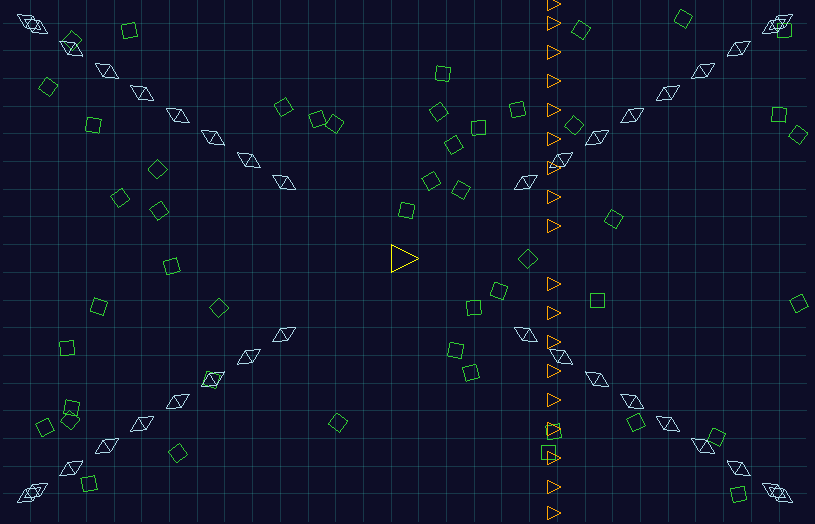
\includegraphics[width=1\columnwidth]{content/de/iterative evolution/img/collisiondetection}
    \caption{Meilenstein 4 beinhaltete die Veröffentlichung der \textit{Enemy Spawn} und \textit{Collision Detection Demo}, die jeweils die Funktionalität des Spawn-Systems und der Kollisionsbehandlung demonstrieren. Der Bildausschnitt zeigt die Spielerfigur (gelb) und die drei verschiedenen Gegnertypen des Spiels.
    Die rhombusförmigen Gegner besitzen eine Chase-Komponente und aktualisieren ihre Bewegungsrichtung in Abhängigkeit von der Position des Spielers. (Quelle: eigene Aufnahme)}
    \label{fig:collisiondetection}
\end{figure}

\subsubsection{Grid-basierte Kollisionserkennung}

Eine weitere fachliche Vertiefung fand in diesem Meilenstein mit der Implementierung des Kollisionssystems statt.
Dieses basiert auf einem Grid-basierten Ansatz (\textit{Spatial Partitioning}), um die Anzahl der zu prüfenden Kollisionen zu reduzieren, und wird in Abschnitt~\ref{sec:systems} beschrieben.